\section{Museum Lighting}

\bigskip

\begin{itquote}{}
Museums and art galleries collect, preserve, and display natural artifacts and/or examples of human achievement and analyze their impact on the world and the universe around us. Effective exhibit lighting must balance exhibition and conservation needs and enrich the museum experience.
\end{itquote}

\begin{flushright}IES RP-30-96 Museum and Art Gallery Lighting: \\A Recommended Practice \citep{ies_ies_1996}\end{flushright}

\bigskip

Lighting in museums is required to satisfy multiple criteria; perhaps the least contestable requirement being that the lighting illuminate objects such that they are suitably visible to museum visitors. Also of utmost importance in most museum settings is that the lighting does not have an unreasonably damaging effect upon the objects or environment, be this through direct photodegradation or as a result of heat transfer. Further to these requirements, an increased or optimal visual quality is generally desirable, although what this represents or how to achieve it is generally ambiguous.

In sweeping terms, all electromagnetic radiation (visible and non-visible) damages objects, and more radiation damages objects proportionally moreso. Thus the question becomes: \emph{how little light can we use to illuminate objects such that they're visible to the extent required?} The inverse form, sometimes used on the assumption that more light always represents an increase in observer satisfaction/pleasure is: \emph{`how much light can we use so that only $x$ damage occurs over $y$ time'}. 

Industry guidance documents provide advice on how to manage lighting to best address the above requirements and many other additional specific requirements through the recommendation of procedure and provision of target figures for quantitative variables. \Gls{UV} radiation, being of no visual benefit but having potential to harm, is now excluded from gallery spaces as an industry standard. %KC: citation required

%KC: I would add a summarising sentence here e.g. "This section discusses existing literature covering the various factors that need to be considered when choosing a museum light source, specifically those that relate to its SPD.  These include the likelihood of damage and the visitor experience.  A discussion of existing museum guidance on these topics is also provided.

\subsection{Damage functions} \label{sec:DamageIndex}

%KC: Can you link this to the ipRGCs?  Overall, this shows that in terms of material damage, the wavelengths to avoid are the low ones and that light sources which have high intensities at the peak sensitivity of melanopsin could be considered as not particularly hazardous for museums.

\textit{The key reference on this subject is \gls{CIE} 157:2004 \citep{cie_cie_2004}, and valuable talks on the subject were given at the recent Museum Lighting Symposium \& Workshops \citep{pokorska_book_2017} (which the author helped to organise), and have been made freely available online\footnote{See in particular the talks by David Saunders (\url{https://www.youtube.com/watch?v=H4d0qH0IBcI&t}) and Stefan Michalski (\url{https://www.youtube.com/watch?v=XUY9biLQqlw})}.}.

\bigskip

In heritage science `damage functions' are ``functions of unacceptable change, dependent on agents of change'' \citep{strlic_damage_2013}. The goal of damage functions in heritage lighting engineering is to give a quantitative means by which to predict the amount of damage caused to a prototypical object by a given light source, and to assist in limiting such damage. They generally follow the logic that radiation of lower wavelength is likely to cause more damage to objects.

\citet{harrison_report_1953} is generally acknowledged as the first to suggest such a function, but he himself acknowledges that it had ``long been established that the shorter the wavelength (visible yellow, green, blue, violet and invisible UV being progressively shorter) the more photochemically potent will be such radiant energy, provided such energy is actually absorbed''. \citet[p.9]{harrison_report_1953} defined the `radiation hazard associated with a light source' as:

\begin{equation}
    \sum_{0}^{\infty} \mathrm{H}_{\lambda} \mathrm{D}_{\lambda} \Delta \lambda / \sum_{0}^{\infty} \mathrm{H}_{\lambda} \overline{\mathrm{y}}_{\lambda} \Delta \lambda
    \label{eq:Harrison}
\end{equation}

where $\mathrm{H}_{\lambda}$ is the spectral irradiance, $\mathrm{D}_{\lambda}$ is the `Relative Damage Factor' (which is extrapolated from the data collected shortly prior to Harrison's own report by the National Bureau of Standards \citep{national_bureau_of_standards_preservation_1951}, and shown in Figure \ref{fig:Harrison}), and $\overline{\mathrm{y}}_{\lambda}$ is the \gls{CIE} 1924 photopic $V_{\lambda}$ luminosity function. The resulting value would describe the amount of damage expected from a light source, normalised by its luminance.

\begin{figure}[htbp]
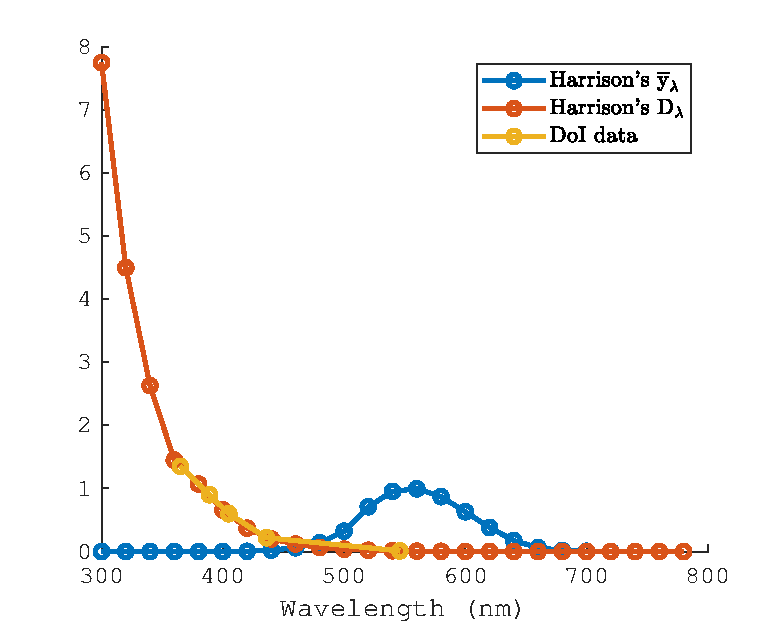
\includegraphics[max width=\textwidth]{figs/LitRev/HarrisonAndDoI.pdf}
\caption{Harrison's \citep{harrison_report_1953} damage function ($\mathrm{D}_{\lambda}$), and luminous efficacy ($\overline{\mathrm{y}}_{\lambda}$), alongside the Declaration of Independence data \citep{national_bureau_of_standards_preservation_1951} from which it was extrapolated (re-normalised to match scale).}
\label{fig:Harrison}
\end{figure}

\begin{figure}[htbp]
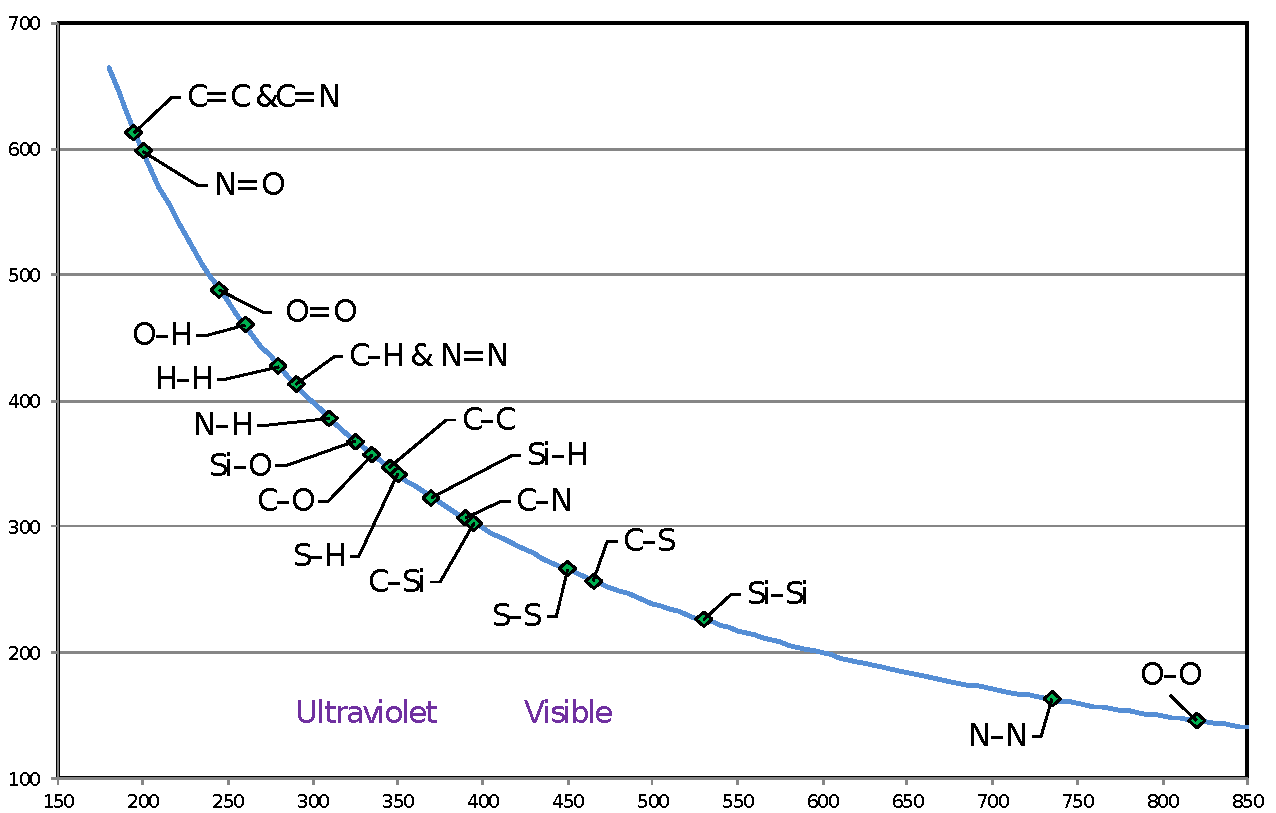
\includegraphics[max width=\textwidth]{figs/LitRev/Saunders.pdf}
\caption{Graph courtesy of David Saunders, presented at the Museum Lighting Symposium \& Workshops \citep[p.61]{pokorska_book_2017} showing the relationship between wavelength and the bonds which can be broken in various molecules, with `Wavelength (nm)' on the abscissa and `Bond energy (kJ/mol)' on the ordinate.}
\label{fig:Saunders}
\end{figure}

There has been extended scepticism about the utility of damage functions in general, with the argument being that no one damage function could represent the vast range and complexities of real materials. \citet[p. 178]{thomson_museum_1978} wrote that ``for more fugitive materials \dots the figure for visible radiation would be higher. On the other hand \dots the fastest dyes are probably affected only by UV. Thus it can be seen that no single figure can be given for damage versus wavelength''.

Criticism was aimed at this specific damage function due to its derivation from such a small and minimally representative dataset - Harrison's data was `extended' from the 5 datapoints measured by the National Bureau of Standards \citep{national_bureau_of_standards_preservation_1951} in their investigations of how to best care for the Declaration of Independence\footnote{It is a curiosity that these minimal figures would not in fact have been much use to those planning the care for the declaration, since in the report it is noted that ``The deterioration of animal parchment is not as rapid as that of the low-grade paper for which the damage factors were determined'' \citep{national_bureau_of_standards_preservation_1951}, and the Declaration of Independence is written on animal parchment.}, and was derived from the study of `low-grade paper', which cannot to said to represent the average museum item\footnote{Though \emph{no} material truly can!}.

\gls{CIE} 157:2004 \citep{cie_cie_2004} notes that whilst Harrison's proposal failed to gain acceptance as the procedure for comparing the damage potential of different types of light sources, it did convince people of the ills of \gls{UV}, with the result that daylight was subsequently eliminated from many galleries.

Following \citet{cuttle_lighting_1988}, who noted that Harrison's damage function could be well fit by an inverted logarithmic function, with parameters controlling the slope and normalisation point of the function, \gls{CIE} 157:2004 provided the following equation:

\begin{equation}
    s(\lambda)_{\mathrm{dm,rel}}=\exp [-b(\lambda-n)]
    \label{eq:damfac}
\end{equation}

where differing values of $b$ for 5 categories of item are provided (Table \ref{tab:b}), $n$ is the normalisation value (\gls{CIE} 157:2004 uses a value of 300), and the $s(\lambda)_{\mathrm{dm,rel}}$ function is the estimated action spectrum for each category. $s(\lambda)_{\mathrm{dm,rel}}$ would be substituted into Equation \ref{eq:Harrison} for $\mathrm{D}_{\lambda}$. \gls{CIE} 157:2004 also provides values of $H_{s,dm}$ which indicate the susceptibility of each group of materials to damage (where damage is considered as colour change%in $\Delta E_{\mathrm{ab}}^{\ast}$
).

\begin{table}[htbp]
\centering
\begin{tabular}{|c|l|l|l|}
\hline
Group & Samples & $H_{s,dm}$ (W h/m$^{2}$) & $b$ \\ \hline
a & Low-grade paper & 5 & 0.038 \\ \hline
b & Rag paper & 1200 & 0.0125 \\ \hline
c & Oil paints on canvas & 850 & 0.0115 \\ \hline
d & Textiles & 290 & 0.0100 \\ \hline
e & Water colours on rag paper & 175 & 0.0115 \\ \hline
\end{tabular}
\caption{Table reproduced from \gls{CIE} 157:2004 \citep{cie_cie_2004}, showing the values for $H_{s,dm}$ and $b$ for various categories. Note: the source for this data is not particularly clear; it is listed as `The Berlin researchers', which is assumed to follow the references: \citet{krochmann_beleuchtung_1988,cie_cie_1991,hilbert_zur_1991}; none of which I have been able to access.}
\label{tab:b}
\end{table}

The more general criticism that damage functions will never be able to represent all museum objects is a valid concern, and can be well illustrated with the following logic: museums own objects of many different colours, different colours arise from different reflectance properties, different reflectance properties mean different wavelengths are absorbed, and damage can only occur when radiation is absorbed. Thus it follows that one would expect two objects of different colours to have different damage functions. 

The classic study on how reflectance properties relate to damage is that of \citet{saunders_wavelength-dependent_1994}. They exposed a number of pigments to a range of wavelengths and measured the resulting damage.%KC: Can you give a bit more detail in this sentence?  Did Saunders and Kirby use a series of monochromatic light sources?  Did damage mean colour change here?
\citet{cuttle_control_1999} later replotted the data from this study (see Figure \ref{fig:Cuttle}), highlighting the apparent joint contributions of spectral reflectance and a general damage function to the individual damage functions. \gls{CIE} 157:2004 notes however that this correspondence is not perfect or easily modellable, and that ``a workable system for characterising action spectra for colorants, including pigments and dyes, remains an unattained goal''. Recent studied have added new data (see esp. \citet{villmann_wavelength_2018}), and it is hoped that a general understanding may at some point be reached.

\begin{figure}[htbp]
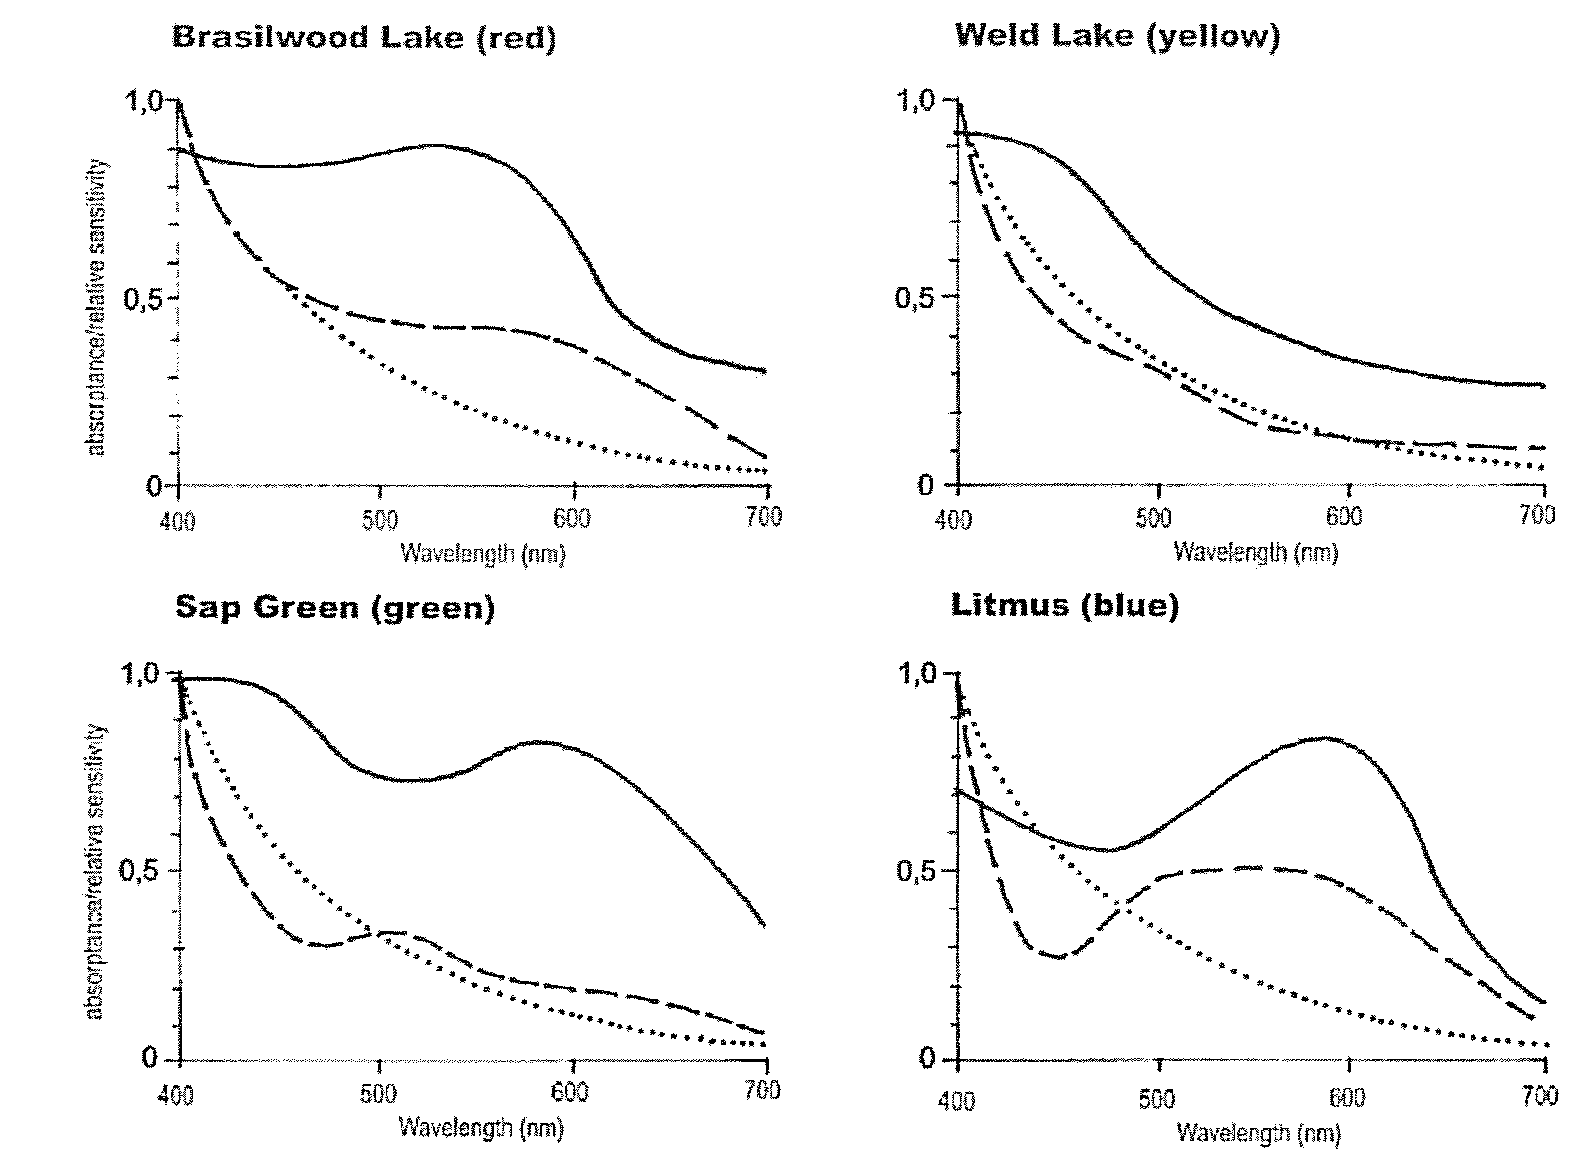
\includegraphics[max width=\textwidth]{figs/LitRev/Cuttle.png}
\caption{The original data for this figure is from \citet{saunders_wavelength-dependent_1994}, later re-plotted by \citet{cuttle_control_1999}, and reproduced (with the addition of the Berlin functions) by the authors of \gls{CIE} 157:2004 \citep{cie_cie_2004}. Caption from \gls{CIE} 157:2004: ``Spectral absorptance (solid line) and relative spectral responsivity (broken line) for artist's pigments \dots The dotted lines show relative spectral sensitivities normalised at 400nm based on the Berlin relative spectral responsivity function.''}
\label{fig:Cuttle}
\end{figure}

However, it is the opinion of this author that this argument is an exercise in artificial futility; whilst we may not be able to model the individual damage functions for every object in a museum, we may at least use one which has some bearing on the damage function, rather than the one which is implicitly used by museums currently - the \gls{CIE} 1924 luminosity function ($\overline{\mathrm{y}}_{\lambda}$ of Figure \ref{fig:Harrison}), which relates to the sensitivity of the human eye rather than any type of object. \citet{cuttle_lighting_1988} puts it well: ``The argument, then, is not whether we have a [damage] function which is correct, but whether we can improve usefully upon the likely reliability of the present system''. It is depressing that this was said in 1988 and yet little seems to have changed in practice (See Chapter \ref{chap:Interviews}).

In the case where specific objects/pigments of interest can be identified, and their individual damage functions calculated, there is valuable research to draw on regarding methods for optimising light sources to minimise damage, initiated by \citet{miller_evaluating_1993} and developed by many others \citep{durmus_optimising_2017,durmus_colour_2015,durmus_optimising_2015,durmus_object_2017,delgado_ramos_art_2009,delgado_lighting_2011,luna_selective_2015,cuttle_proposal_2000,vazquez_point_2017}. The fading of lead chromate in the paintings of Vincent van Gogh has captured public attention \citep{lewis_smith_will_2013} and has resulted in multiple studies looking at ways to optimise the illuminant for this one particular material \citep{lunz_can_2017,monico_degradation_2011}.

With modern computation, and access to datasets, it becomes relatively easy to calculate a value of \Gls{DI}. Figure \ref{fig:Houser} shows the results for such computations for 401 illuminants and light sources (as per Equation \ref{eq:Harrison}, using a damage factor computed as per Equation \ref{eq:damfac}, but further normalised such that Illuminant A has a reference value of 1)\footnote{The code to reproduce this is available from: \url{https://github.com/da5nsy/DamageIndex}}. It can be seen that whilst most illuminants cluster around 1 there is a broad range. It should be remembered that these illuminants would in no way indicate their relative damage index to an observer or a purchaser, unless one went to the effort to look up or measure the \gls{SPD} and compute the damage factor. A careful or careless choice in this respect could easily double or halve the amount of time an item could be exhibited before succumbing to terminal damage.

\begin{figure}[htbp]
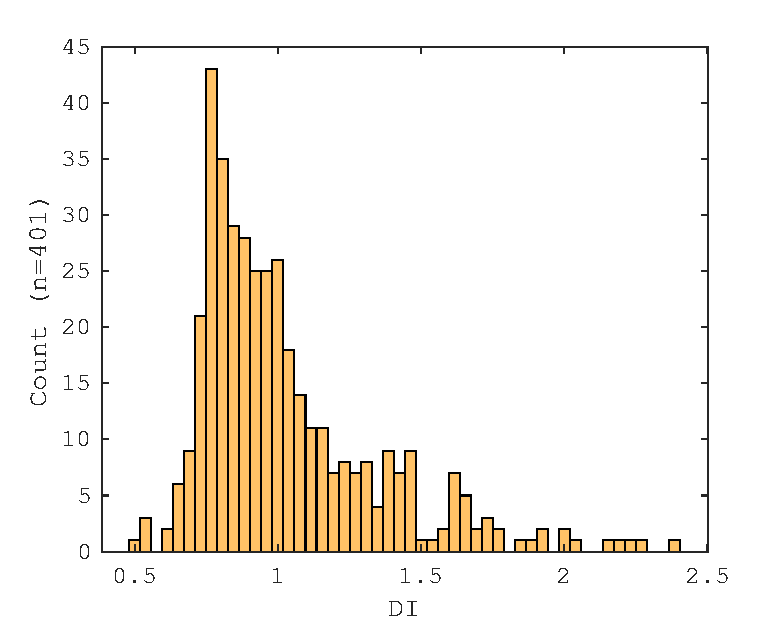
\includegraphics[max width=\textwidth]{figs/LitRev/DI.pdf}
\caption{The values of $DI$ for the 401 illuminants used by \citet{houser_review_2013}, available via \gls{PTB} as `spd\_houser', normalised such that \gls{CIE} Illuminant A receives a reference value of 1.}
\label{fig:Houser}
\end{figure}


\clearpage
\subsection{Visitor Requirements of Museum Lighting}

The visual requirements of museum visitors is likely to depend upon a large number of variables, both intrinsic and extrinsic to the visitor (e.g. intrinsic - age, cultural background, goals for the museum visit and extrinsic: luminance, lighting distribution, \gls{CCT}, \gls{CRI} and flicker properties of lighting). Some of these factors have been independently studied in a museum context, and for others it is likely that findings in other environments could generalise such that they could be used to inform decisions regarding museum lighting.

Traditionally, the principal manner in which museum professionals sought to limit damage was through setting a maximum luminance level. The implicit assumptions in this process are twofold; firstly: that damage will increase with increased luminance. This was a fairer assumption when tungsten was the only type of lighting technology, but as other lighting technologies with different \glspl{SPD} have been introduced this assumption has become less accurate (see Section \ref{sec:DamageIndex}: \nameref{sec:DamageIndex}). The second implicit assumption is that viewers will prefer higher luminance environments.

The classic study on this second assumption, performed in a mock-museum environment is that of \citet{loe_preferred_1982}. This research regards the display of oil and watercolour paintings specifically. In this study Loe et al. examined three variables: painting illuminance, light source (different technologies) and light distribution. Following the construction of a mock up gallery space, observers were asked to view paintings of various types under a range of illuminations, varying in `painting illuminance, light source and light distribution within the gallery space' and report upon semantic scales their perceptions. The results which informed the 200 lux recommendation stem from only the first variable, painting illuminance. Here it was found (as shown in Figure \ref{fig:Loe}) that for factors christened `discrimination' and `quality evaluation' (distilled from factor analysis of the original semantic data) there was `a steep rise in discrimination and quality assessment until and illuminance of approximately 200 lux is reached: above this illuminance the rate of increase in reduced.' This conclusion has had substantial impact in setting guidelines and future thinking was that a minimum of 200 lux was required to `give visual satisfaction', however it can be seen from Figure \ref{fig:Loe} that the data is sparse, noisy, dependent upon brand of illuminant and doesn't show a particularly strong effect of 200 lux in particular. Further, only a small number of different luminances were sampled, and it is quite possible that the results are at the mercy of several types of bias \citep{fotios_research_2009}. This figure was subsequently used in \citet{thomson_museum_1978}, which has informed a great deal of subsequent thinking on the topic.

\begin{figure}[htbp]
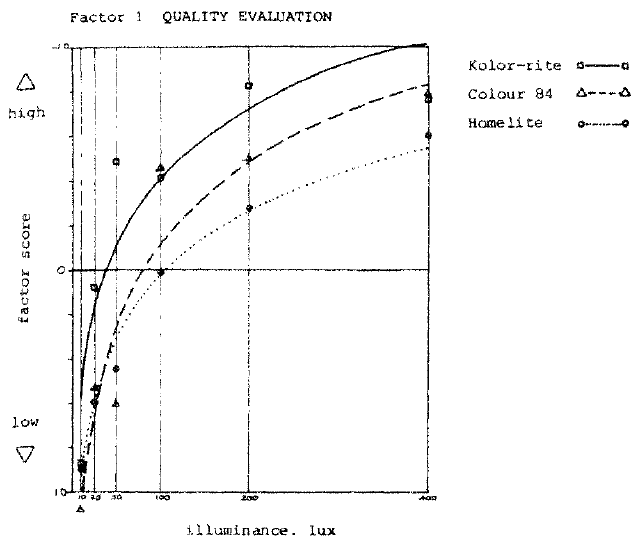
\includegraphics[max width=\textwidth]{figs/LitRev/Loe.png}
\caption{Illuminance vs a factor which is thought to indicate `quality', for three different brands of illuminant, reproduced from \citet{loe_preferred_1982}.}
\label{fig:Loe}
\end{figure}

There has been extensive research on the visitor requirements in terms of \gls{CCT} and \gls{CRI} and these shall be covered in separate sections.

In terms of a holistic approach to museum lighting research (considering more than a single or small number of isolated variables), there has been a great deal of work which deals with the visitor experience in a broad and cultured fashion from the lofty vantage of museum studies (such as \citet{falk_museum_2016} and \citet{shapiro_museum_1990}), but rarely do the physical practicalities such as lighting get a mention. 

The notable exception, where lighting as it relates to the visitor experience is considered, is the work of Kesner in the USA in the early nineteen-nineties \citep{kesner_museum_1993-1,kesner_museum_1993,kesner_exhibition_1992,kesner_current_1991,kesner_analysis_1997}.

Kesner's studies comprised self-reporting surveys, and concluded that colour accuracy was the highest requirement and that `richness' of colour was the lowest priority\footnote{A cautious interpretation of these results is advised, considering that there were high average scores for each category.}:

\begin{citequote}{kesner_museum_1993-1}
Artifact appearance, particularly clarity of artefact form and accuracy of artifact color, is the most important visitor need. Although visual impression, specifically acceptable gallery brightness and rich artefact color, is least important among the factors, it too rated highly important.
\end{citequote}

%more?

%Following the release of guidelines on the topic of \glspl{LED} in museums \citep{druzik_guidelines_2012}, a written survey of museum professionals who had requested these guidelines was performed, and the results reported by \citet{perrin_ssl_2014}. The respondents were predominately based in USA, with 30\% identifying as `international'. The survey was part of the USA government's `GATEWAY program'. Responding to the question `Please rank the following factors in your selection of lamps', joint first priorities are identified as `colour and spectral power distribution' and `damage potential'.

\subsection{Museum Lighting Specification Guidance Documents}

\textit{For a historical perspective on museum lighting guidance see \citet{druzik_museum_2007}.}

Five museum lighting guidance documents, thought to represent the most referred to documents in the field (informed by the interviews reported in Chapter \ref{chap:Interviews}), were reviewed. 

The purposes of this section:
\begin{enumerate}
\item To explore how museum professionals specify lighting, by understanding the tools and guidance which are available
\item To enquire as to what the guidance actually is, in terms of what subjects are covered and what the guidelines actually are
\item To question what these guidelines are based upon. How are the results of scientific study utilised in the production of these documents?
\end{enumerate}

Limiting the damage to museum objects by photodegradation is most often the responsibility of the preventive conservator within a museum, or the person holding a role which encompasses this role in the case of smaller institutions. It is therefore essential that the people in these roles have access to standardised and validated advice on how to approach the subject. Several overviews of the subject have been written and I shall aim to introduce the most prominent here, focusing on their aims, scope and differences/similarities. 

I shall operate a biased interest towards the recommendations regarding colour rendering, colour temperature, and illuminance level. Whilst the first two are the immediate area of study within this project, the third (luminance) is of interest for multiple reasons. Firstly, it is the most prominent area in which lighting guidance is provided, on the assumption that there exists a correlation between illuminance and damage, and secondly because of the unit of specification- lux, which is generated using a function of wavelength designed to provide a correlate of brightness to humans. As a human based function, it is within the scope of interest to this project.

There shall be an active occlusion of any advice, no matter how interesting, pertaining to subjects other than lighting and to areas of lighting guidance which do not fall into the above remit, such as directionality, UV/IR damage, advice relating to specific technologies and areas of discussion such as cost calculations or warranty considerations. 

Firstly, a general note regards the mind-set of those providing recommendations: conservation recommendations provided to museums, which might be presumed to be concerned with a method for limiting damage, are generally in no way informed by the sensitivity of a prototypical object, nor how light might act upon it, but rather it is concerned with maintaining a minimal acceptable light level for an observer to view objects under.

This is based on the argument as follows: all light is damaging, but required in order for visitors to see objects. Damage by light acts in a roughly reciprocal manner, such that a small amount of light over a long time period might be made to do equal damage as a large amount of light over a short period. Considering the multiple aims of museums; (1) to display objects, but also (2) preserve them such that they may be displayed to future generations, it seems desirable to find the minimal amount of light that satisfies the first aim, such that the ability to deliver on the second aim is maximised. Thus many of the recommendations discussed here are actually concerned with the ability of a viewer to extract visual information. This point is not always entirely clear, and it is my suspicion that conservators are sometimes lulled into believing that there is something special about the specific values recommended regards their ability to `avoid' damage. 

One clear exception to this, which will be discussed in further detail, is \gls{CIE} 157:2004 \citep{cie_cie_2004} which considers damage functions of specific materials. These deal specifically with the degradation of objects, with less regard to how objects might appear. Other works which deal with damage functions either generally or for specific types of objects fall into this exception also.

The common language most regularly employed in both of these approaches is the term of 'lux', though this is a contentious issue with some arguing that it correlates well enough with damage potential, and others exploring the use of damage functions. `Lux' relates loosely to the human perception of brightness, but does not consider any type of material absorbance, reflectance or damage function. The historical background to this precedent appears to be as follows; whilst technological ability to vary the spectral power distribution of a light source was limited (whilst tungsten was the dominant source of illumination) is could be assumed that there was a predictable relationship between lux and radiometric spectral power distribution, such that any two lights with the same lux level would cause the same level of damage to any specific object, and thus providing damage minimisation advice could be done using the language of lux, which was pre-established considering the original approach outlined above. This approach is now less appropriate, considering the increased variability in spectral power distribution provided by the introduction of LED technology, and it is reasonable to assume that in the future additional lighting technologies (or variations of existing technologies) might be introduced, with again fundamentally different types of spectral power distribution.

This field may be divided into publications which relay original research, generally in the form of journal articles and conference proceedings, and longer publications which aim to provide an authoritative voice on the subject (often including references to the aforementioned journals). I shall cover principally these longer documents, since my priority interest in this section is the advice which is currently provided and the methods in which this advice is conveyed. The question of how much conservators rely on guidance documents vs referring to ongoing research is an interesting question in of itself, and shall be covered in my discussion of the interviews conducted with current museum professionals (See Chapter \ref{chap:Interviews}).

\noindent
The guidelines chosen for review were:
\begin{itemize}
\item The Museum Environment \citep{thomson_museum_1986}
\item \gls{CIE} 157:2004 Control of Damage to Museum Objects by Optical Radiation \citep{cie_cie_2004}
\item Guidelines for Selecting Solid-State Lighting for Museums \citep{druzik_guidelines_2012}
\item SLL LG8: Lighting for museums and art galleries \citep{cibse_lighting_2015}
\item IES RP-30-96 Museum and Art Gallery Lighting: A Recommended Practice \citep{ies_ies_1996}\footnote{This has since been usurped by IES \citep{illuminating_engineering_society_ies_2017}.}.
\end{itemize}

\noindent
In summary:
\begin{itemize}
\item Recommended values were provided for:
\begin{itemize}
\item \emph{Lux}: various, dependent on sensitivity, generally based on figures from the study of visual preference by \citet{loe_preferred_1982} via \citet{thomson_museum_1978}.
\item \emph{R$_a$}: various, most frequently \textgreater 80, generally with no experimental basis referenced or justification for this exact figure.
\item \emph{\gls{CCT}}: various, based implicitly on \citet{kruithof_tubular_1941} or on such ideas found empirically.
\end{itemize}
\item Most also suggested visual inspection as a valid means of assessment.
\item There was often blurring between recommendations concerned with visual appearance and those concerned with conservation. 
\end{itemize}

\subsubsection{`The Museum Environment'}

`The Museum Environment', first published in 1978 \citep{thomson_museum_1978}, with a popular second edition published in 1986 \citep{thomson_museum_1986} (I shall hereon be referring to this later edition), appears to be one of the most frequently consulted resources on the subject of lighting for practising museum professionals. Whilst the book encompasses a great many subjects aside from lighting, two chapters are set aside for the subject of lighting specifically, covering a large range of topics within the scope of museum lighting. In Druzik's overview of museum lighting specification \citep{druzik_museum_2007} he notes that `up until the first edition of The Museum Environment in 1978, no one had written a book on preventive conservation in museums that was comprehensive, yet clear enough for scientists and conservators to use with nearly equal ease.'

The section of Thomson's book most often referred to in my experience has been his guidance on recommended exposure for different object types. A table from this section is reproduced below as Figure \ref{fig:Thomson} which details the types of objects which might most readily be assumed to fall into groups of like sensitivities. The recommended maximum illuminance values stem most heavily from experiments performed by \citet{loe_preferred_1982} in the years immediately previous to the publication of this second edition. It is noted that these recommendations are a revision upwards from the first edition, where 50/150 lux was recommended in place of 50/200 lux.

\begin{figure}[htbp]
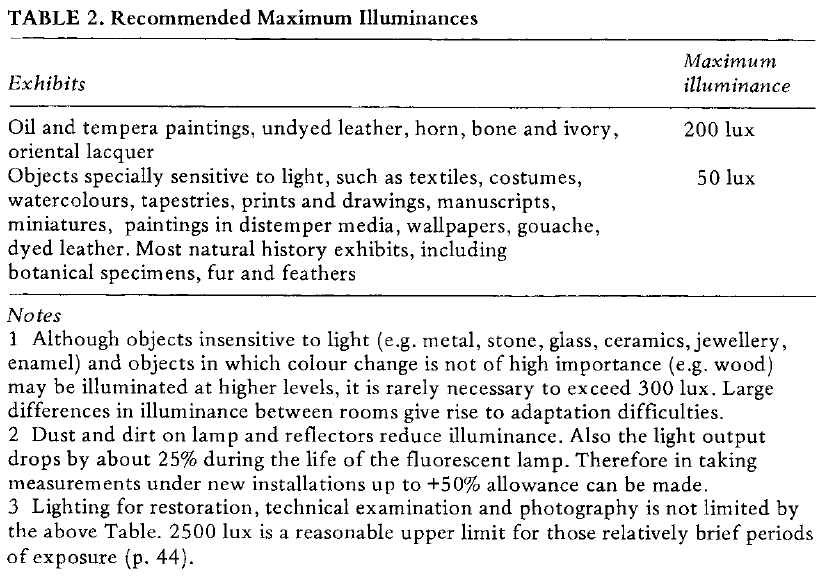
\includegraphics[max width=\textwidth]{figs/LitRev/Thomson.png}
\caption{Table 2 of \citet[p. 23]{thomson_museum_1986}, describing recommended maximum illuminances for 2 groups of objects.}
\label{fig:Thomson}
\end{figure}

Loe et al.'s work concludes with the recommendation that ``preferred artificial lighting conditions for viewing works of art are a painting illuminance approaching 200 lux provided from lamps with good colour rendering characteristics, e.g. a \gls{CIE}~R$_a$ index of \textgreater 85 and a large gamut area''. It is of particular interest to me that Thomson neglected to quote the final part of this recommendation regarding the specific \gls{CIE}~R$_a$ and note regards gamut area.

On the topic of colour rendering, Thomson goes into great depths to explain the topic and the means available for calculating various indices, spending a disproportionate amount of time (compared to what I understand was normal for the time) on the topic of Crawford's `band method' \citep{crawford_colour_1960,crawford_measurement_1959} for colour rendering index calculation amongst other things.

For the most part he neglects to make recommendations for specific target values, only making the rough and unsupported assertion in passing: 

\begin{itquote}{}
Recommendation for good colour rendering. \\
\gls{CIE}~R$_a$ about 90 or better, \\
R\textsubscript{w} (worst R) about 80 or better, \\
and Crawford Class A, B or C
\end{itquote}

No research is referenced to support this recommendation. The inclusion of $R$\textsubscript{w} (the lowest value of $R$\textsubscript{i}) is notable due to its lack of consideration in other documents. 

Still on the topic of colour rendering, of additional note is Thomson's general introduction to the subject, where he frames the conversation in a manner which presents colour rendering as a measure of the colour changes to which the human visual system is unable to adapt to, opposite changes induced by changes in colour temperature to which the human visual system is generally able to adapt easily to. Thomson also provides an accessible, and often quoted summary of the underpinnings of how the \gls{CIE} General Colour Rendering Index operates in principle:

\begin{itquote}{}
Adapt our eyes to the illuminant under test. \\
Look at a set of representative objects under it and accurately memorise their colours.\\
Adapt to the reference illuminant.\\
Look at the same objects under this second illuminant and compare the colours to the colours in our memory.
\end{itquote}

Thomson's comments on the selection of colour temperature are minimal, not referring to any specific \gls{CCT} in his summary of specifications [p. 268]. The only note dealing directly with the specification of colour temperature can be found on page 25, and refers only specifically to the conversation of what colour temperature to select for those environments which for conservation purposes need to be lit at particularly low illuminance levels.

\begin{itquote}{}
The `coolness' \dots of daylight when it has been reduced to 50 lux often gives the impression of gloom, especially when it is highly diffused. No one knows how deeply it has been built into our systems, but ever since our first ancestors sat around fires, and later used oil lamps and candles, the human race has been accustomed to `warm' light in the home after dark. As a result the warm 50 lux from tungsten lamps appears to be brighter, and certainly more cheerful, than 50 lux of diffused daylight. For the same reason warm rather than cool fluorescent lamps should be chosen for 50 lux situations.
\end{itquote}

It is assumed that the views expressed above are grown from empirical observation. They mirror the standpoint of other publications which refer to the work of \citet{kruithof_tubular_1941} and the derived `Kruithof curve' (see Section \ref{sec:CCTmus)}).

The bulk of pages 49-51 concern colour temperature, if one includes the associated discussion of chromatic adaptation and colour constancy, but there is no clear link as to how the author suggests that this theory should be considered in practical application, nor any concrete recommendations for target figures.

A final note in reference to this text goes to the discussion of whether or not to consider the type of lighting for which the artist intended an artwork to be displayed under, or that under which it was originally created. At the risk of quoting half the book I include one final passage which I think particularly pertinent to the area of research to be undertaken in this project, with which I shall conclude my discussion of this publication:

\begin{itquote}{}
I think one would be correct to suppose that artists have always assumed that their creations would be viewed in a variety of situations, not all lit ideally, and have designed their work accordingly. Even the Impressionists and others who made a point of completing their canvasses in the open air did not expect them to be so viewed. When De La Tour painted a candle-lit scene he painted it in such a way that the scene would look candle-lit under any reasonable lighting (for a contrary view see Weale [\citep{weale_truth_1973}]). 

But it could also be said that, however robust the work of art, it will look better in some lighting situations than in others, and so we should bend our efforts to finding the best possible situation. Within the limitations of the museum one cannot but agree, provided there is indeed a consensus of perceptive opinion on what is best, and provided that the damage caused by light is kept under control. 

There is certainly no mathematical treatment whereby we can equate the viewer's gain against the exhibit's loss. However there has been considerable research on the visual process as it is affected by the lighting, and Brommelle [\citep{brommelle_visual_1972}] has carefully related the experimental work to the museum problem.
\end{itquote}

\subsubsection{\gls{CIE} 157:2004 Control of Damage to Museum Objects by Optical Radiation}

This document is a \gls{CIE} technical report, prepared by \gls{CIE} Technical Committee 3-22 of Division 3 ``Interior Environment and Lighting Design''. 

To set the context for the discussion of this \gls{CIE} technical report, first a note to draw attention to the time period during which it was drawn up, since to the future reader there might be some ambiguity as to what the state of the art was at this point. Whilst it is now at the time of writing in 2016 common to find museums using LEDs to display their objects, this was not the case in 2004. It is noted within the text that LEDs are `are not of suitably high colour quality for museum use at present, but have future potential as very low UV power sources.' The increased use of LEDs does not invalidate the contents of this document, but it is worth considering that it was prepared with pretext to address any LED specific issues.

As previously mentioned, this document takes a different approach to the problem of limiting light induced damage in museums, focusing rather on the process of considering the optimal spectral power distributions as opposed to limiting the light levels wholesale. For example, the closest the document comes to making light level recommendations in the manner of `The Museum Environment' \citep{thomson_museum_1986} is in the tabulation of Mlx hour values for predicted noticeable fade. This approach leaves the decision of actual lighting levels to the museum professionals, with the question being `How long do I want this object to last before a noticeable fade has occurred?'

The document is in some ways an endorsement and extension of the approach taken by \citet{harrison_report_1953} (as discussed in Section \ref{sec:DamageIndex}), in which the concept of a damage function was introduced, this being ``an action spectrum that defines the relative spectral responsivity of a receiving material''. The authors of this document note that the work did not originally gain traction due to conservators' scepticism that a single function could represent the vast range of potential museum object (still an intractable problem). Interest was further lessened by the fact that the original work refers only to one very specific type of material - low grade paper. However, the authors of this document argue that the fundamental idea is sound; a damage function (so long as it is genuinely representative to an extent) could be a valuable tool in assessing the appropriateness of different light sources.

The authors then pull reference from further studies focused on a range of other materials, and find low grade paper is actually an outlier in terms of wavelength sensitivity, with many other materials able to be grouped together in type of dependency (if not like sensitivity). Following Cuttle's work \citep{cuttle_lighting_1988} to describe the pre-existing damage functions as simple mathematical relationships, comparison between the variety of newly created damage functions was possible.

Regarding colour temperature, the report states:

\begin{itquote}{}
While the variations of spectral responsivity for individual materials, particularly pigments, remains problematic, the overall tendency for responsivity to increase at shorter wavelengths is reasonably well defined. It has been shown that there is a general effect for the relative damage potential to increase as colour temperature increases [\citet{cuttle_lighting_1988}]
\end{itquote}

This falls short of offering recommendations for colour temperature choice, remaining impartially scientific. However, an included table, reproduced below, makes it clear that the lower the colour temperature, the lower the potential for damage (for a set SPD `type').

\begin{figure}[htbp]
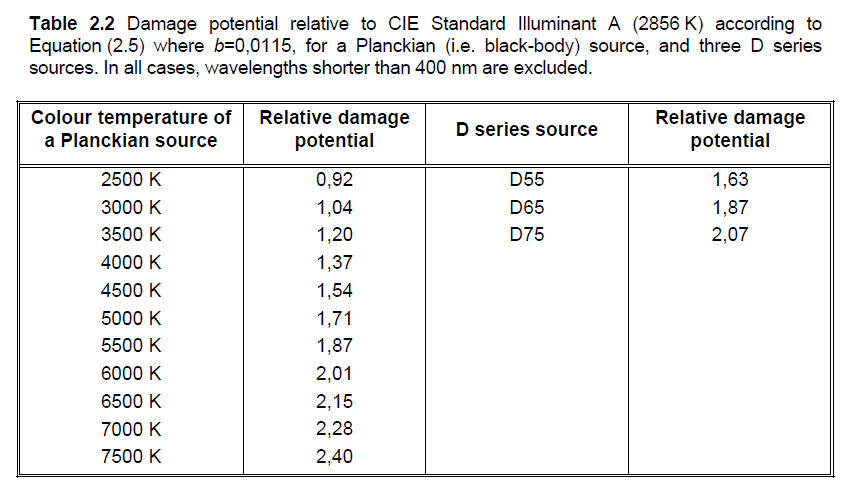
\includegraphics[max width=\textwidth]{figs/LitRev/CIE2004b.png}
\caption{Table 2.2 of \gls{CIE} 157:2004 \citep{cie_cie_2004}}
\label{fig:CIE2004b}
\end{figure}

This section concludes with the introduction of two related topics, again with significance for this project. The first regards the work of \citet{miller_evaluating_1993} in which the concept of `reflected energy matching (REM)' is introduced, the second is of the work by \citet{thornton_high_1975} in which he describes the technique of using `prime colour' light sources.

REM in the current context refers to a process of illuminating an object preferentially with illumination of wavelengths which it is known to reflect. The premise of this is: absorbed radiation is visually unimportant, yet conversely the radiation most likely to damage an object. Thus an ideal situation would be to illuminate an object with radiation which it entirely reflects. The immediate limitations of this process are that this process would be object specific and potentially problematic for correct colour rendering. This procedure was suggested to be implemented using fibre optics and filter systems, it would likely be much more approachable with the advent of LED technologies which allow certain spectral flexibility.

A note in the text regards the potential for REM to increase the saturation of colours relates that this `raises questions concerning the ethics of modifying the apparent colours of displayed objects.' 

\hl{Thornton/Prime}
\hl{(Colour rendering/critical viewing)}

In the final section of this document (written with the aim to `give recommendations for lighting in museums') very little advice is given in the form of specific figures to aim for, rather a decision appears to have been made that it was preferable to detail the areas that the authors considered worthy of attention, and to lay out the arguments for deliberation. For example, on the topic of \gls{CCT} choice reference is made to the previous discussion which details the deleterious potential of illumination at different colour temperatures, but it is clearly stated that `[w]here the viewing conditions call for moderate or high colour temperature lighting, conservation concerns should not override design objectives for the display.' This seems to be supported by the later statement that `[i]t is thoroughly bad policy to place an object on display, where it inevitably will suffer some damage, and to fail to present it adequately.' It is further noted that low colour temperatures may `judged unsatisfactory' when it is used in combination with natural illumination. 

With marked separation, the previously discussed work of \citet{loe_preferred_1982} is referred to, in the context of providing guidance on a lux value that is `generally sufficient to provide for adequate visibility'.

There is a noteworthy section on the meaningful distinction between illuminance and irradiance: `It needs to be recognised that illuminance is not a reliable alternative measure [for irradiance], as it represents the density of luminous flux, being radiant flux evaluated according to a typical human visual response, defined by the photopic spectral luminous efficiency function V($\lambda$). Not only does illuminance take no account of irradiance outside the visible spectrum, but also radiant flux within the visible spectrum is weighted according to its relative visual effect, which is not related to its damage effect.'

\subsubsection{CGI/Getty Guidelines for Selecting Solid-State Lighting for Museums}

This guidance document \citep{druzik_guidelines_2012}, produced by the Canadian Conservation Institute and The Getty Conservation Institute, provides guidance for museum professionals to select \gls{LED} lighting. As such, the guide includes an introduction to the technological theory of \glspl{LED}, advice on how to consider the requirements of museum lighting, and a practical guide to selecting lighting. It is the only document here considered which discusses solely LED technology.

Compared to the other documents considered here, there is also a focus on the longevity of systems, particularly in respect to potential for colour change, and advice on the type of information that should form a warranty agreement between supplier and end user.

A recurring piece of advice throughout the document is that a lighting specifier should always view lighting in person before making a significant order. The implicit, and sometimes explicit subtext here is twofold; firstly, that the specifications available for lighting are insufficient to describe the visual appearance of lighting, and secondly, that the quality of museum lighting (the ability of lighting to fulfil predetermined requirements) is visually assessable. An extension of this second point would be to consider the visual requirements in museums as being solely or principally defined by a general preference for appearance under lighting.

Following this notion, \gls{CIE}~R$_a$ is referred to as `imperfect' and `misunderstood', and it is suggested that it could be used as a `secondary consideration'. There are several different specific values of \gls{CIE}~R$_a$ recommended at different points within the document.

\begin{itquote}{}
It is generally agreed that a \gls{CRI} above 85 is suitable
\end{itquote}
\begin{itquote}{}
To illuminate areas with a more utilitarian [function] such as machinery, many science exhibits, food services, hallways, educational activities, etc. settle on a color rendering index (\gls{CRI}) above 80. When color matching may be more an attentive activity such as viewing art, ethnography, some natural history collections exhibits, etc. select \glspl{LED} with a \gls{CRI} above 90. However, because \gls{CRI} is an imperfect metric, \gls{CRI} should be considered a target, not a firm criterion.
\end{itquote}
\begin{itquote}{}
There is no international museum standard on what is or is not an ``acceptable'' \gls{CRI}, but the Canadian Conservation Institute (CCI) recommends a minimum of 85. Many museums specify greater than 90.
\end{itquote}

As is perhaps apparent in the quotes above, this document has the feel of friendly advice rather than an official guidance document. As such, it has particular value for this project as a perhaps more revealing account of the advice which actually circulates in the field. For example, one piece of advice which I haven't seen anywhere else in official literature, but which as I understand it is relatively common in general parlance is that provided during the overview on page 23: `Check color rendering on your own skin'. This advice is incongruous with the museum lighting advice which prioritises objectivity and impartiality, as this implicitly suggests looking for a `pleasing' appearance.

The document makes subtle references to the \gls{CQS} \citep{ohno_rationale_2010,baier_is_2012,davis_toward_2005,davis_color_2010} and \gls{GAI} \citep{rea_color_2008}; saying that in response to limitations with \gls{CIE}~R$_a$ `at least two other color metrics have been proposed recently', followed by references which relate to the aforementioned respectively. The document also makes two references specifically to \gls{CIE}~R$_9$ values, firstly as part of the information on the ENERGY STAR program (where it is quoted alongside other lamp specifications) and once in the Appendix (where visual demonstrations of induced colour shifts are provided for the \gls{CQS} and \gls{CIE} test colour samples. Interestingly, a scale for \gls{CIE}~R$_9$ is described, where: `\gls{CIE}~R$_9$ = 0-49 means it renders red hues well. When R9 is 50-74 it is very good. R9 above 75 is considered excellent.' As with many items in this document, no reference as to the source of this information is provided. 

Regards the question of CCT within museum lighting, the guidance offers a Kruithof-ian approach, though without naming it as such, recommending warmer light for lower light levels and colder light for higher light levels. 

\begin{itquote}{}
With low light levels, as in museums, viewers tend to prefer warmer light similar to that of incandescent lamps, e.g. the 2800K of standard incandescent lamps, or the slightly higher 3000K of quartz halogen incandescent lamps. As illumination increases to several thousand lux, preference is for cooler light, 5000K or higher.
\end{itquote}

It is noted than an exception might be made in the situation where artificial lighting is employed to augment natural illumination. This said, elsewhere in the same document the reader is advised to `avoid higher color temperatures for light sensitive materials as these LEDs may have an unacceptably large peak in the ``blue region'' of the spectrum.'

Also poorly referenced is the discussion of the 50 lux recommendation. Research is mentioned but not directly quoted. It is assumed that the research described as `in the 1980s' is the previously discussed research of \citep{loe_preferred_1982}.

The final area of note within this report is that which considers the methods applicable to assessing museum lighting in situ. A survey completed at the Field Museum \citep{myer_demonstration_2010} is quoted in detail, the survey having been completed by museum staff and lighting practitioners as part of a GATEWAY program demonstration at the museum. This survey includes such questions as `The lighting product shows \underline{\hspace{2cm}} of the subject colors accurately' and was completed for a halogen system and an LED system in the same space.

\subsubsection{SLL LG8: Lighting for museums and art galleries}

\citet{cibse_lighting_2015}

% To be written up
% -	Recent doc 2015
% -	Benefits from Practical examples
% -	Lots of big/familiar names
% -	Limited references, no in line sources

% -	Pg 3 CCT warmer light standout?
% -	Pg 4 CRI 90 very good, <80 not suitable
% -	5 colour of backgrounds
% -	9/12 combining daylight and cct
% -	24 `purely advisory' reflect current practice
% -	25 `access has two components, visibility and duration of exposure to light'
% -	27 basing on `good eyesight' might be `discriminatory'
% -	28 distorting intention of artist
% -	33 V&A JNC 50years?
% -	43 trade off
% -	46 blue peak ongoing research
% -	47 essential to conduct side-by-side trials
% -	67 good colour quality = poor efficacy?
% -	Many specific object types

\subsubsection{IES RP-30-96 Museum and Art Gallery Lighting: A Recommended Practice}

\citet{ies_ies_1996}

% -	1996, as of 2016 being updated
% -	Guide for lighting designers

% -	1 `human achievement'
% -	1 Different priorities for different people (kesner)
% -	1 Three rules
% -	2 `Color should not change the look of an artifact' ``overriding – original appearance''
% -	3 CRI ``true color'' >80
% -	3 CCT Determine whether the display takes on a warm or cool appearance
% -	12 30lux required for color
% -	12 avoid bold surrounding colours
% -	13 `killing the patient'
% -	15 lux = exposure(?)
% -	31 Brief history of daylight in galleries
% -	31 adaptation



















\subsection{CCT in museums}
\label{sec:CCTmus}

\Gls{CCT} is often described as an important variable in museum lighting, but definite recommendations, in the rare cases that they are given, are generally based on nostalgia for the appearance of tungsten lighting, questionable research on human preference \citep{kruithof_tubular_1941,fotios_revised_2017} or very rough rules that predict that damage potential will be decreased if \gls{CCT} is minimised \citep{cie_cie_2004}. Whilst some research appears to have found optimal \glspl{CCT} for viewing artwork \citep{nascimento_best_2014,pinto_correlated_2008,scuello_museum_2004,scuello_museum_2004-1, liu_cultural_2013,vidovszky-nemeth_introductory_2016,feltrin_impact_2019} results often have large inter-observer variability, context dependency and it is not uncommon for the headline findings of separate studies to be in contradiction. 

Specifications often refer implicitly or explicitly to the findings of \citet{kruithof_tubular_1941}, who found that at lower levels of illumination, lower \glspl{CCT} were preferred, and that at higher levels of illumination higher \glspl{CCT} were preferred (see Figure \ref{fig:Kruithof}). Whilst this general trend seems to have anecdotal support, it is possible that there may be lighting-technology-based confounds, and recently researchers \citep{vienot_kruithofs_2009} (including a meta-study of multiple other examinations \citep{fotios_revised_2017}) found there to be no substantive support for Kruithof's findings.

% Kruithof is referred to a lot but needs proper discussion somewhere. %DG: I think I do that already above (?)

\begin{figure}[htbp]
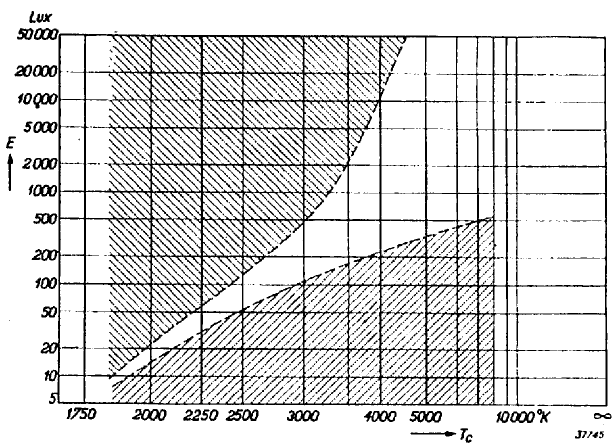
\includegraphics[max width=\textwidth]{figs/LitRev/Kruithof.png}
\caption{The `Kruithof curve' reproduced from \citet{kruithof_tubular_1941}, showing colour constancy against illuminance, and highlighting an area that is considered ``pleasing'' (central white area).}
\label{fig:Kruithof}
\end{figure}

The damage justification seems more substantive; following the application of damage factors as discussed in Section \ref{sec:DamageIndex} the \gls{CIE} published a report showing the varying the \gls{CCT} of museum lighting could have a clear impact on the potential damage undergone by museum objects \citep{cie_cie_2004}. 

\begin{figure}[hbtp]
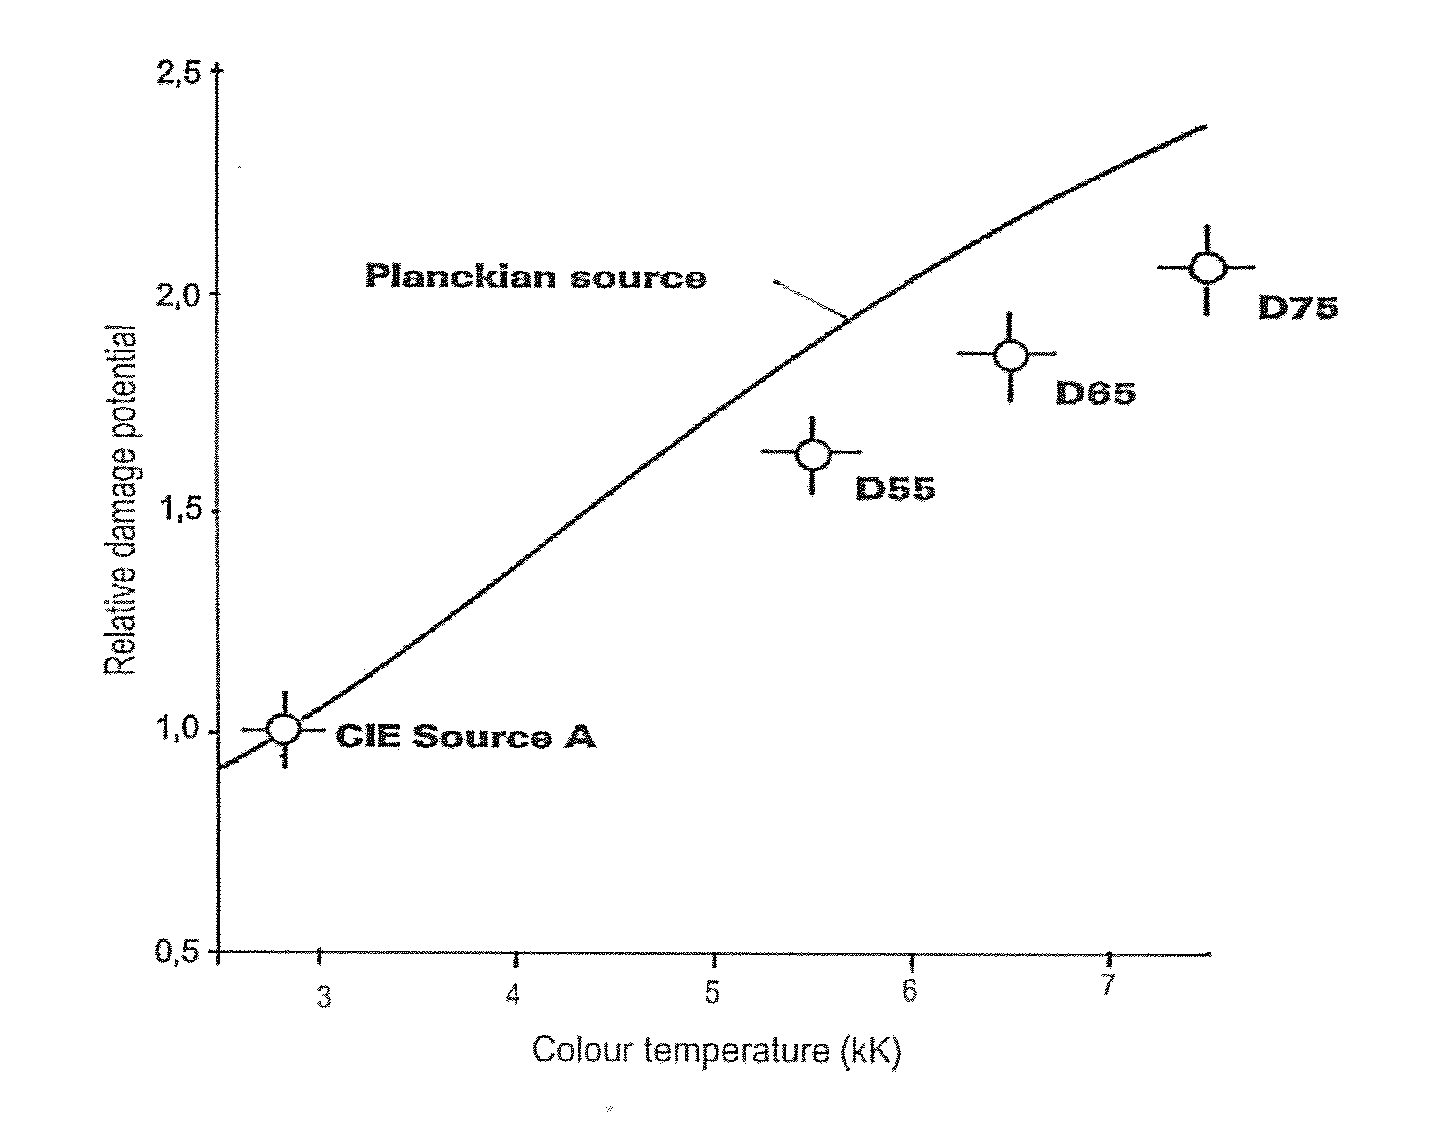
\includegraphics[max width=\textwidth]{figs/LitRev/CIE2004.png} 
\caption{Figure reproduced from \gls{CIE} 157:2004 \citep[p.16]{cie_cie_2004}, showing the relationship between \gls{CCT} and relative damage potential for black body radiator illuminants, \gls{CIE} source A and three \gls{CIE} D-series illuminants.}
\label{fig:CIE2004}
\end{figure}

This line of reasoning relies heavily upon the applicability of damage functions to the specific materials in question. As discussed previously (Section \ref{sec:DamageIndex}) it seems that whilst the generalised damage functions account for some of the individual material damage functions, they do not fully do so. However, tentatively, they do seem to be a relatively good fit for the shared characteristics of different damage functions (at least far more so than V($\lambda$)), and so it seems reasonable to use them where no other broad approximation for a large set of objects exists.

To verify the findings of the \gls{CIE}, extend their findings to \glspl{LED}, and provide code for others to do similar research or even test their own lights/materials, a set of MATLAB functions\footnote{\url{https://github.com/da5nsy/DamageIndex/blob/c7851e27ca1b0915013d8723db04704b49b4085e/CalcDI.m}} have been written by the author which calculate \gls{DI} values for arbitrary illuminants. This code has been used to produce Figure \ref{fig:CCTvsDI}, which shows the \glspl{CCT} and \glspl{DI} of the 401 \glspl{SPD} of \citet{houser_review_2013}. A $b$ value of 0.0115 corresponding to `oil paints on canvas' and `water colours on rag paper' (see Table \ref{tab:b}) was used. It can be seen that there is a clear correlation between \gls{CCT} and \gls{DI} with higher \glspl{CCT} being predicted to be relatively more damaging. If a damage function with a lower $b$ value (such as for `low-grade paper' or `textiles') had been used, the relationship between \gls{CCT} and \gls{DI} would be steeper.

%\afterpage{\clearpage}
%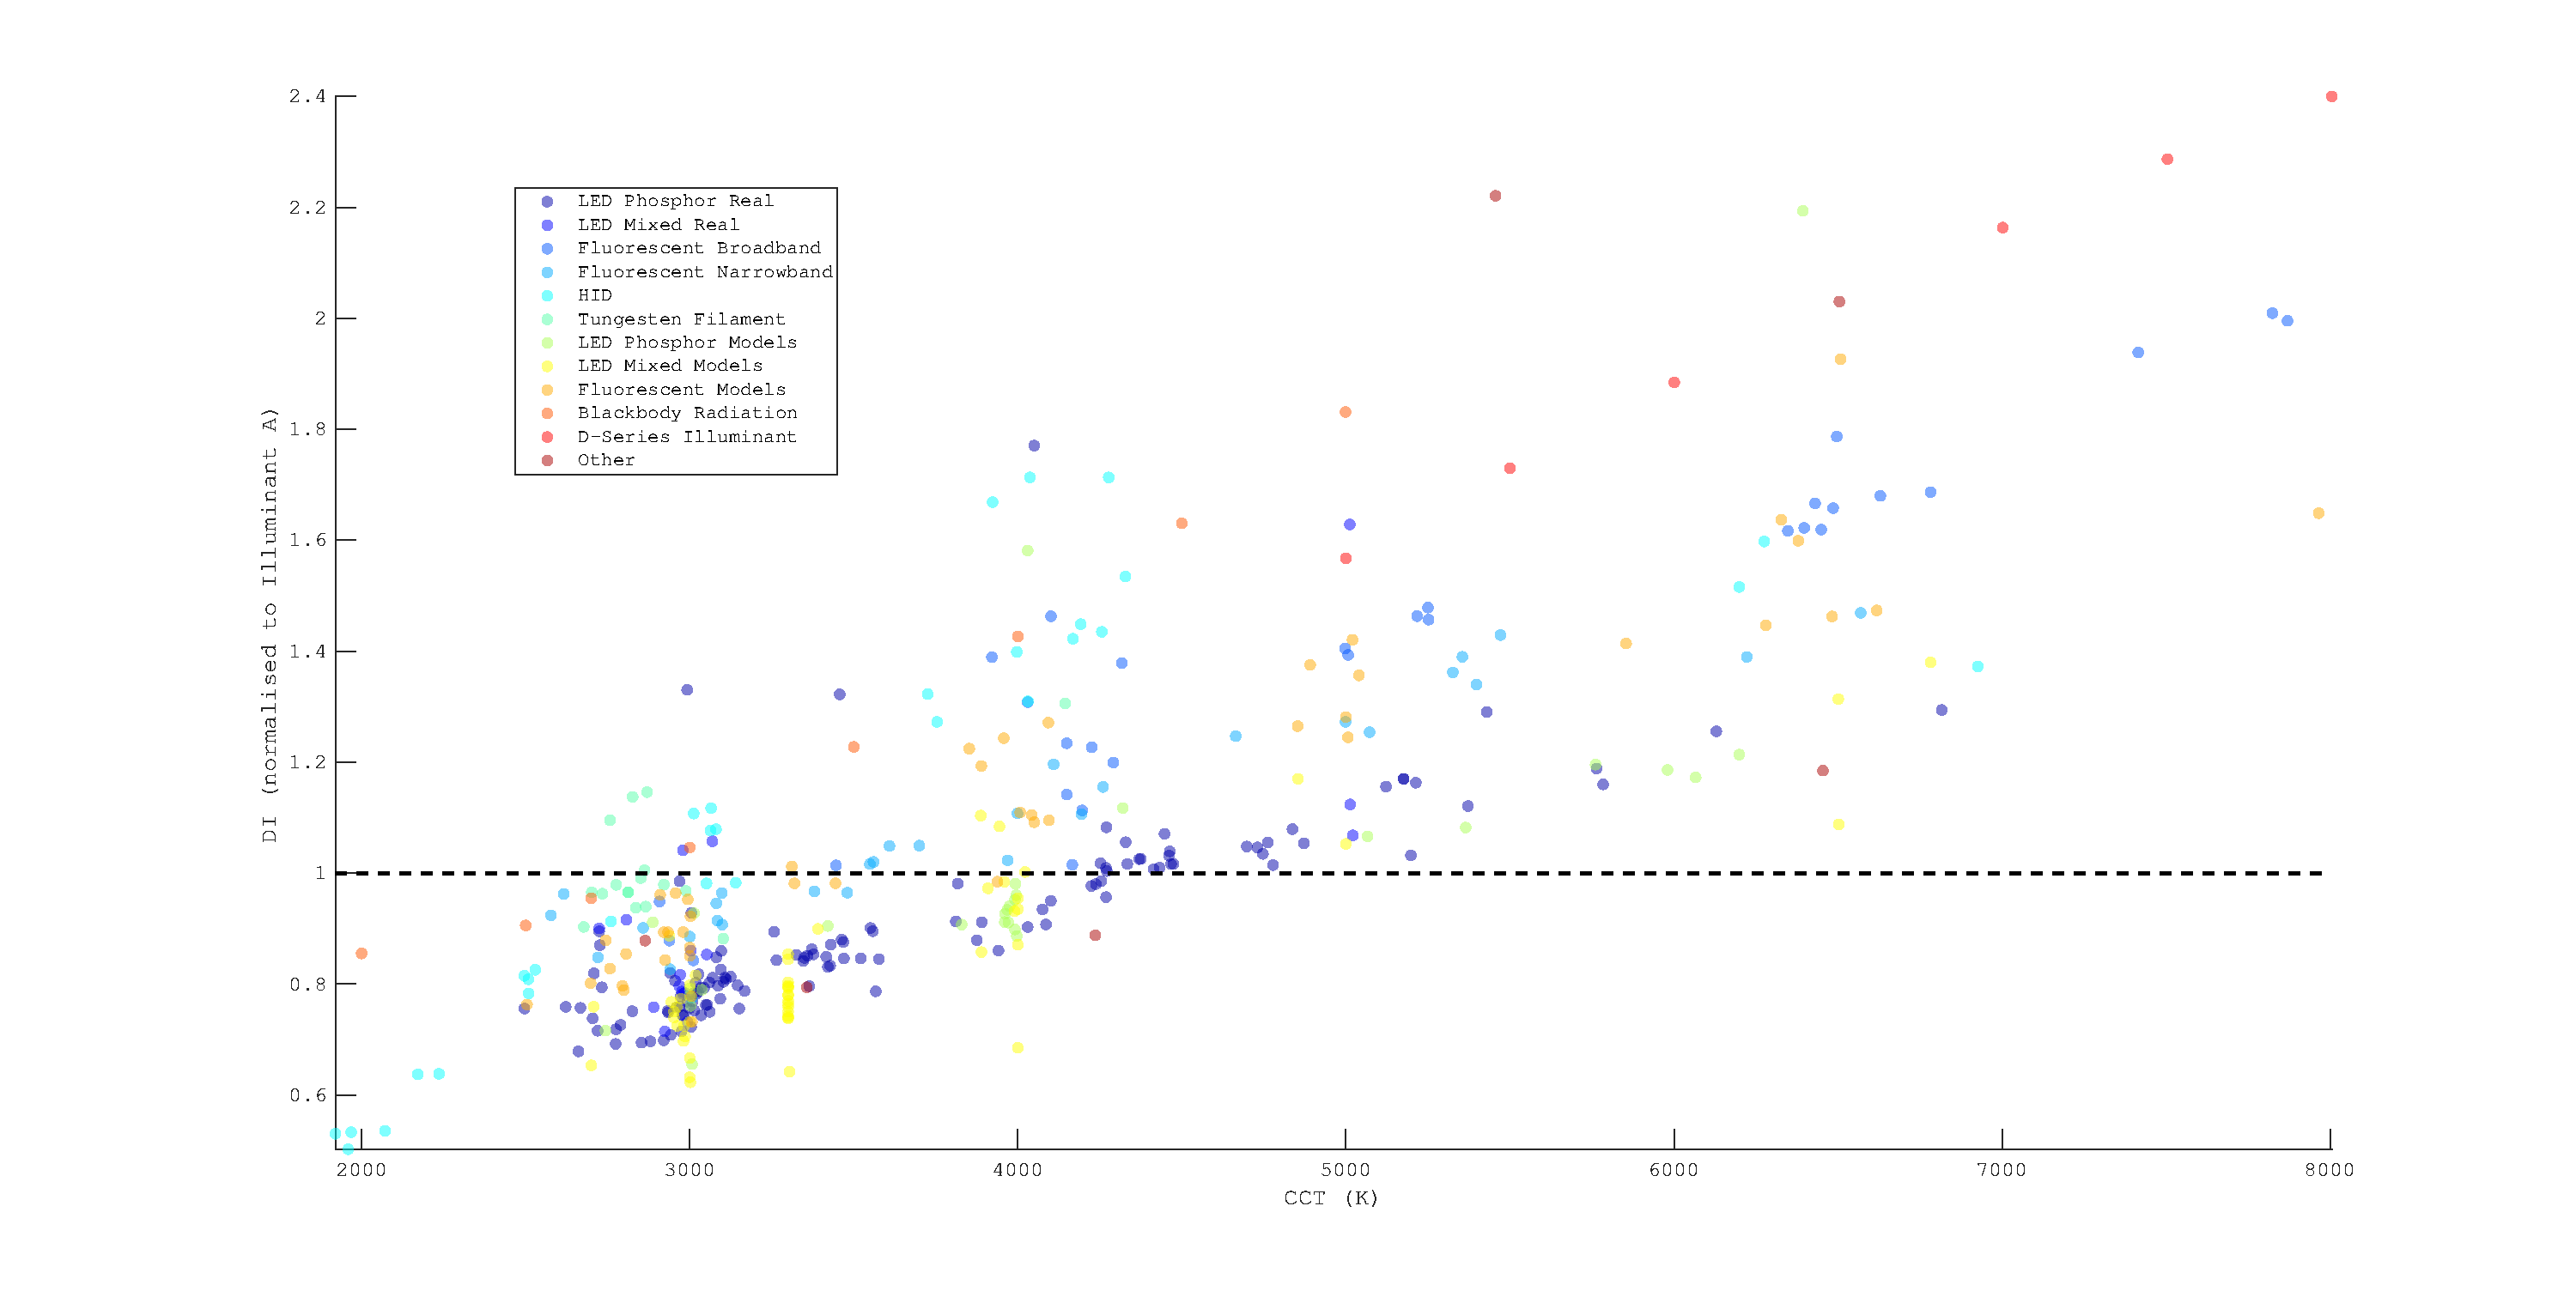
\includepdf[pages=-,rotate=90, offset=75 -75]{figs/LitRev/CCTvsDI.pdf}
% \begin{figure}[t]
%     \caption{The \glspl{CCT} and \glspl{DI} of the \glspl{SPD} used by \citet{houser_review_2013} [provided via personal communication, but now partially available via \gls{PTB} as `spd\_houser'].}
%     \label{fig:CCTvsDI}
% \end{figure} 

\begin{fullpagefigure}
\figpdf[pages=-,rotate=90, offset=-85 -85]{figs/LitRev/CCTvsDI.pdf}
\figpageside{}
\caption{The \glspl{CCT} and \glspl{DI} of the \glspl{SPD} used by \citet{houser_review_2013} [provided via personal communication, but now partially (without category information) available via \gls{PTB} as `spd\_houser'].}
\label{fig:CCTvsDI}
\end{fullpagefigure}

The results of these computations show a clear relationship between \gls{CCT} and \gls{DI}. Considering that this is not currently taken advantage of in museum lighting, it seems as though there is a great potential for reducing damage whilst maintaining visitor visual satisfaction.

%\clearpage
% This is combo with the figpageside thing above currently isn't quite working

%%%% !!!!!!!!!! Check this works before printing

\cleardoublepage %works but seems a bit heavy handed.

\subsection{Colour Rendering Indices in Museums}

%Are fidelity indices suitable for museum use? 
The first chapter of Cuttle's book `Light for Art's Sake: Lighting for Artworks and Museum Displays' \citep{cuttle_light_2007} is titled `A philosophy for the presentation of art'. The choice of title here is apt but may surprise some readers, sounding more whimsical than might be expected of a serious subject attended by scientists and engineers. The reason it is so apt is because lighting is unavoidably a creative intervention\footnote{Credit for this phrase to Katherine Curran} which is to say that there is no lighting which is truly impartial, and no lighting which is truly `correct' in the sense of being unequivocally superior to another. All lighting decisions require choices to be made, and whilst these choices can be wrapped up to appear as an optimisation problem where proximity to a particular solution is the goal, the problem always rests on the bedrock of a philosophy based decision.

In the above mentioned chapter Cuttle lays out a total of seven distinct philosophical propositions, which he poses for consideration as approaches to museum lighting, some contradictory and some with the potential to overlap:

\begin{enumerate}
\item To make the artwork appear as it would have appeared to the artist at the time of its creation
\item To ensure that no damage due to light exposure will occur
\item To achieve the best possible appearance of the artwork
\item To provide optimum conditions for viewing art
\item To impart a sense of having seen `the real thing'
\item To assist viewers to understand the displayed objects and their reason for being there
\item For the lighting designer to establish a distinct and recognisable style
\end{enumerate}

These propositions refer to museum lighting holistically, considering all aspects of museum lighting, but can be readily focused on the problem of colour appearance specifically. Before we narrow our gaze however, it is worth briefly considering a wide view of lighting attributes which may aid in the realisation of `good quality' museum lighting. Consider Rosenfeld's list of the five `controllable qualities' in museum lighting; `intensity, movement [temporal artefacts], angle [modelling, avoiding glare and reflections], distribution [ambient lighting vs. spot lighting], color' \citep{rosenfeld_agony_2013}.

Whilst Cuttle's propositions make for interesting discussions and enjoyable extended pondering, they are of limited assistance in the practical task of actually specifying lighting. Thankfully, a range of tools exist for the examination of the colour rendering properties of a light source, in the form of indices which aim to numerically describe an illumination's effect on colour appearance of the objects of which it is tasked with illuminating.

Traditionally, colour rendering indices aim to offer a standardised method for calculating the colour differences induced by the substitution of a reference illuminant with a specific test source, and for comparing the relative merit of different test light sources on their ability to induce minimum change. In modern parlance this type of index should be referred to as a colour fidelity index, that is - one which is conceptually concerned with colorimetric reproduction. The term `colour rendering' has come to encompass much more than just fidelity.

Diametrically opposed in some ways to fidelity are the indices which aim to quantify `preference'. In the simplest case, a preference index will aim to provide a value that is predictive of how an observer would rate a light source against other light sources. 

Within and between these two groups there exist a range of different indices with subtly different aims and mechanisms for achieving these aims. For thorough overviews see \citet{guo_review_2004} and \citet{houser_review_2013}.

In practice, both of these philosophical approaches are mandated in current lighting guidance. For the most part, advice for lighting specification on the subject of colour rendering can be simplified to read `use lamps of above \gls{CRI} 80 (referring tacitly to \gls{CIE}~R$_a$) but always test them visually before you buy in bulk'. Whilst this may at first seem like sensible advice, upon further inspection it actually represents a serious contradiction, unless considered with heavy caveats. The problem rests in the fact that \gls{CIE}~R$_a$ is a fidelity index, whereas any visual inspection is likely to be performed by observing the appearance of an object under the test illumination without a reference. Fidelity aims to describe accuracy of reproduction, but this is a quality which is arguably not testable by visual inspection. This contradiction seems to perpetuate unnoticed in museum practice, with lighting specifiers often abstractly declaring to target a faithful/accurate/honest/impartial representation of objects, but practically choosing light sources based on visual inspection where preference is the only criteria. There is of course a range of approaches, ranging from pure reliance on indices to almost entire reliance on visual testing.

In conclusion, no one metric exists that would satisfy the divergent aims and philosophies of museum lighting. Several distinct types of colour rendering index exist, but the existing range fall into the broad categories of `fidelity' or `preference', with the latter being particularly poorly definable due to its variability in different environments, with different user functional requirements and different intrinsic preferences between different observers. Progress could be made by breaking these broad categories into smaller more manageable specific objectives.

%weale_truth_1973

%vienot birds
% vienot_leds_2011

%bespoke colour rendering indices, sistine chapel
% schanda_new_2014

%correcting for hunt effect
% wei_consideration_2018



%%%% BONUS AREA %%%%%%%%%%


%\subsection{LEDs in museums}

%%%%%%%%%%%%%%%

%Theoretically, there exists a division between recommendations which deal with visual appearance and those which deal with physical degradation; the first group supported by the science of human vision, and the second supported by material sciences and chemistry. Whilst it is important to be aware of this distinction, it is normally not possible to consider them entirely separately in practice, as many variables will affect both.

%%%%%%%%%%%


%Extending the question of visibility is the subject of appearance. It is a general expectation that museums represent objects in a truthful and impartial manner, and it seems sensible that decisions concerning the appearance of items in museums should be made with this in mind. Alongside this, many museums treasure items where part of their value is aesthetic2, and it follows therefore that a technique which aids in the beautification of an object might be of interest, and this might be particularly of interest if the object is known to have deteriorated since the time of production.

%%%%%%%%%%%

% \subsection{Lighting at The British Museum}

% Lighting at the British Museum has developed in a somewhat organic manner, from the early days of the museum before the introduction of artificial lighting. This leaves the museum with more than sufficient daylight in most spaces during daylight hours, where the increased modern knowledge regarding the deleterious effect of lighting now means that conservators must find ways in which to limit this natural resource so that objects are not unduly exposed. 

% The gallery lighting is replaced when a gallery is refurbished, and the latest technology is installed when a new gallery is created, where viable in terms of suitability and considering financial limitations. Other than this, lighting technologies tend to not be updated other than to replace individual lamps. This coupled with the grand scope of the museum, which means that it is rare for multiple galleries to be refurbished simultaneously, has led to a vast array of lighting designs and technologies. It in fact appears to represent a rather special example of `museum lighting through the ages', with daylight, tungsten, fluorescent and metal halide lamps all seemingly represented, as well as various illumination geometries reminiscent of the times of their fitting. It should be noted that these assertions are made following empirical observation with spectrophotometers and not from conversations with museum staff, see section 3.3 Collection of \gls{SPD} Data at British Museum.

% There also seems to be a great range of lighting quality within the British Museum, with some spaces feeling bright and others comparatively gloomy. There is a range of colour temperatures and chromaticities of light at the museum, as shown in Figure 1.

% Multiple methods are currently employed to limit the exposure of objects in the museum. \Gls{UV} absorbing film or glazing which incorporates \gls{UV} reduction is used throughout the museum and in certain galleries there are automatic blinds which limit the intrusion of direct sunlight at specific times of the day and year. For particularly sensitive objects, rooms are lit artificially at very low levels, and some objects are selectively lit in order to further limit their accumulative exposure.

% 